\documentclass[preprint,12pt]{elsarticle}
\usepackage{amsmath,amssymb}
\usepackage{booktabs}
\usepackage{threeparttable}
\usepackage{tabularx}
\usepackage{array}
\usepackage{graphicx}
\usepackage{microtype}
\usepackage{xcolor}
\usepackage{enumitem}
\usepackage{siunitx}
\usepackage{url}
\usepackage{hyperref}
\usepackage[capitalise,noabbrev]{cleveref}
\usepackage{lineno}
\usepackage{multirow}
\usepackage{longtable}
\usepackage{pdflscape}
\newcolumntype{L}{>{\raggedright\arraybackslash}X}
\newcolumntype{R}{>{\raggedleft\arraybackslash}X}
\newcommand{\code}[1]{\texttt{#1}}
\newcommand{\forum}{LabAutomation.io}
\newcommand{\repositoryurl}{https://github.com/fraware/lab-automation-observatory}
\newcommand{\pilotnote}{All quantitative results are bounded pilot estimates from purposively selected cases.}
\hypersetup{colorlinks=true,linkcolor=black,citecolor=blue!55!black,urlcolor=blue!60!black}
\setlist{nosep,leftmargin=*}
\sisetup{detect-all=true}
\Urlmuskip=0mu plus 2mu\relax
\emergencystretch=2em

\begin{document}
\begin{frontmatter}
\title{Supplementary Material for ``Where Laboratory Automation Work Breaks''}
\author{Mat\'eo H. Petel}
\end{frontmatter}

\renewcommand{\thetable}{S\arabic{table}}
\renewcommand{\thefigure}{S\arabic{figure}}
\renewcommand{\thesection}{S\arabic{section}}

\section{Taxonomy and code boundaries}
The complete machine-readable taxonomy is provided in \path{data/derived/taxonomy_rules.csv}. B1 and B10 are ecosystem conditions and become primary codes only when knowledge governance or support is the central object. B2--B9 are technical constructs with explicit inclusion and exclusion rules.

\section{Evidence register}
The public derived register contains 55 threads. It records titles, dates, primary and direct-support codes, evidence type, public outcome, migration, evidence strength, source URL, and analytical note. It excludes user handles and a verbatim corpus.

\begin{table}[t]
\centering
\caption{Direct-support and primary-code counts in the selected 55-thread register.}
\label{tab:code-counts}
\begin{threeparttable}
\begin{tabular}{@{}lrr@{}}
\toprule
Code & Direct support & Primary \\
\midrule
B1 & 32 & 1 \\
B2 & 18 & 10 \\
B3 & 18 & 8 \\
B4 & 13 & 7 \\
B5 & 17 & 5 \\
B6 & 11 & 6 \\
B7 & 12 & 6 \\
B8 & 19 & 4 \\
B9 & 5 & 3 \\
B10 & 48 & 5 \\
\bottomrule
\end{tabular}
\begin{tablenotes}[flushleft]\footnotesize
\item Coding is multi-label by design, so direct-support counts sum to more than 55. Exactly one primary code is assigned per thread, so the primary column sums to 55.
\item B1 and B10 are cross-cutting ecosystem conditions. Their high direct-support counts reflect deliberate modifier coding and purposive selection, not prevalence.
\end{tablenotes}
\end{threeparttable}
\end{table}


\section{Episode register}
The difficult subset contains 45 episodes from 14 threads. Each episode records its lifecycle stage, primary code, modifiers, evidence form, detectability, consequence, public artifact, counterexample status, and coding confidence.

\section{Hard-case adjudication set}
\label{sec:s-adjudication}
All coding was performed by one analyst, so no inter-rater statistic is reported. The release instead publishes the prepared adjudication set in \path{data/derived/reliability_subset.csv}. It covers the same 14 threads that were segmented into episodes and records, for each thread, the expected primary code, the most plausible competing code, why disagreement is likely, the specific adjudication question, whether episode segmentation is required, and a priority. Twelve threads are marked critical and two high.

The file is an instrument rather than a result. A second coder can code the listed threads independently, answer the recorded adjudication questions, and then compute agreement on the primary code and on episode boundaries without renegotiating the coding task. Publishing the expected disagreement surface before any second pass also prevents a later agreement statistic from being computed only on the unambiguous threads. No agreement coefficient appears anywhere in this release because no independent second coding exists.

Because the expected primary code sits in the same row as the source URL, the key cannot itself be used for a blind pass: a coder who opens it to find the thread has already read the answer. The release therefore also publishes the generated projection \path{data/derived/reliability_subset_blind.csv}, which carries only the thread, its source URL, the adjudication question, the expected episode count, and the priority. A second coding pass uses the blind sheet; the key is reserved for adjudicating the result afterwards.

\section{Metric definitions}
\subsection{Integration Accessibility Score}
For known component scores $s_j\in\{0,0.5,1\}$,
\[
  \mathrm{IAS}=\frac{1}{|K|}\sum_{j\in K}s_j,
\]
where $K$ is the set of publicly known applicable components. Unknown components are reported separately.

\subsection{Reproducibility Manifest Completeness}
For applicable manifest fields $M$,
\[
  \mathrm{RMC}=\frac{1}{|M|}\sum_{j\in M}s_j,
\]
where 1 denotes immutable binding, 0.5 denotes partial representation, and 0 denotes omission from the reviewed evidence.

\subsection{Physical Definition Completeness}
PDC uses the same field mean over identity, geometry, material, tolerance, coordinate semantics, nesting, operating properties, provenance, validation, and reproduction. Evidence grade is reported independently.

\subsection{Observability Coverage}
OC is the known-field mean over linked run/configuration, material, command, acknowledgement, observation, state change, failure, intervention, recovery, and final disposition.

\subsection{Preflight Preventability}
Complete-case PPR is the number of definitely preflight-preventable scenarios divided by the sum of definitely preventable and definitely non-preventable scenarios. Indeterminate cases define sensitivity bounds.

\subsection{Pairwise association}
For the two-by-two table $(n_{11},n_{10},n_{01},n_{00})$,
\[
  \phi=\frac{n_{11}n_{00}-n_{10}n_{01}}
  {\sqrt{(n_{11}+n_{10})(n_{01}+n_{00})(n_{11}+n_{01})(n_{10}+n_{00})}}.
\]

\section{Validation-stage representation}
The AI method-generation result in the analyzed discussion was reported at one stage only. \Cref{fig:s-validation-funnel} separates that stage from the stages that were described without a denominator and from the stages that were not reported at all, so that the depth of the reported evidence is visible without inference. The stage rows and counts come from \path{data/metrics/ai_validation_funnel.csv}, whose interval columns are recomputed by \code{labauto\_observatory.metrics.wilson\_interval}.

\begin{figure}[tp]
  \centering
  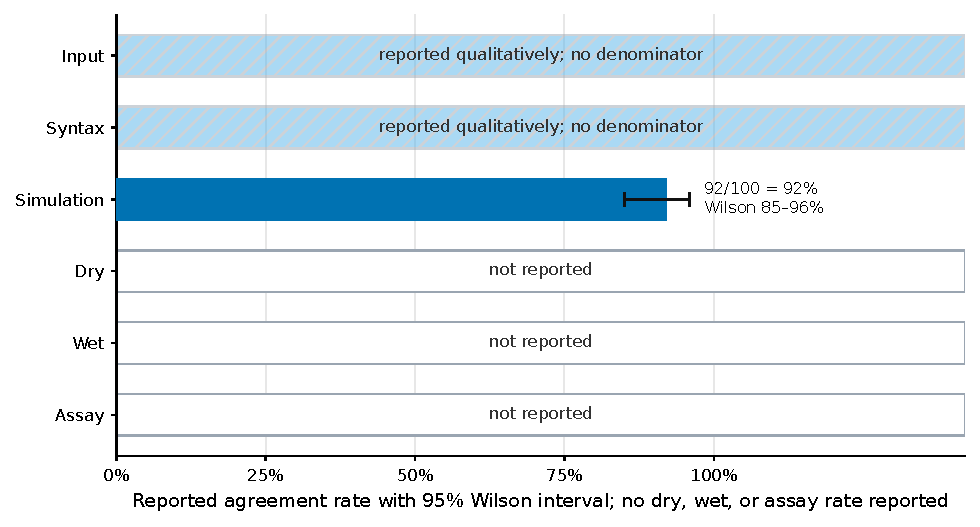
\includegraphics[width=0.94\linewidth]{figures/validation_funnel.pdf}
  \caption{Validation-stage representation for the source-reported AI method-generation result. Only the simulation stage carries a denominator, so only that stage is drawn as a rate with an interval. Stages that were described without a denominator, and stages that were not reported at all, are drawn as bands across the whole axis rather than as bars, so that ``reported'' cannot be read as a measured success rate.}
  \label{fig:s-validation-funnel}
\end{figure}

\section{Test--claim alignment elements}
A claim counts as fully aligned only when all five elements support the normalized statement, so the class in \path{data/metrics/b8_test_claim_alignment.csv} is determined by the element scores rather than asserted alongside them. \Cref{fig:s-b8-alignment} shows which element is missing in each partial or incomplete case, which is the information the headline proportion necessarily discards.

\begin{figure}[tp]
  \centering
  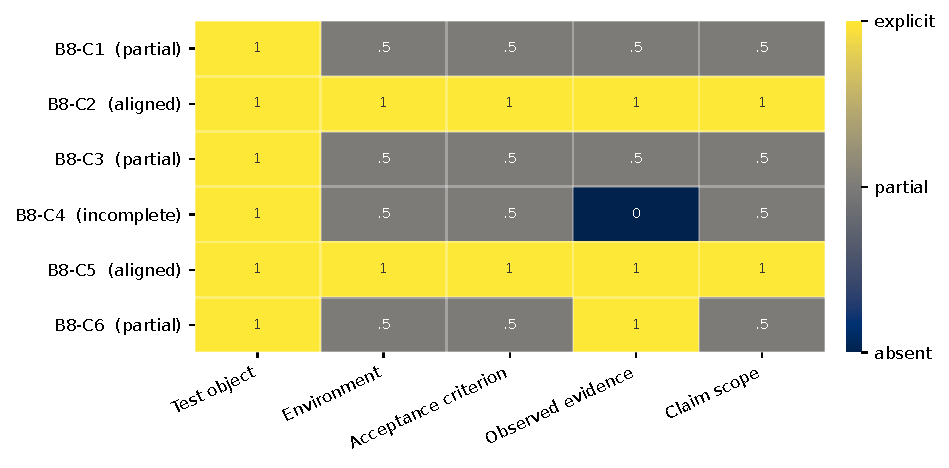
\includegraphics[width=0.94\linewidth]{figures/b8_alignment_matrix.pdf}
  \caption{The five alignment elements for each of the six bounded B8 test claims. Every claim named a test object; observed evidence and reconciled acceptance criteria were the elements most often left partial. The row label records the overall alignment class assigned during coding.}
  \label{fig:s-b8-alignment}
\end{figure}

\section{Preflight preventability and its bounds}
The complete-case Preflight Preventability Rate has a denominator of three, so the point estimate carries very little information on its own. \Cref{fig:s-b6-preventability} therefore shows the four eligible scenarios and their detectability classes beside the rate, its Wilson interval, and the two values the rate would take if the indeterminate scenario were resolved in either direction. The indeterminate scenario is never imputed.

\begin{figure}[tp]
  \centering
  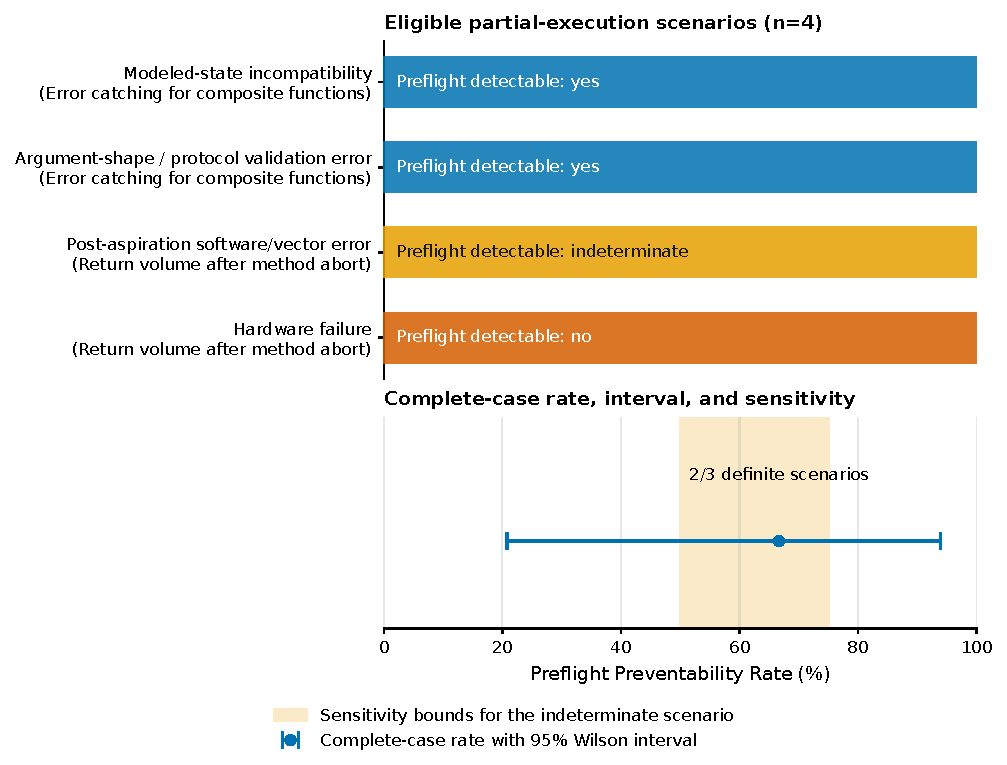
\includegraphics[width=\linewidth]{figures/b6_preflight_preventability.pdf}
  \caption{The four eligible partial-execution scenarios by preflight detectability, beside the complete-case rate. The complete-case denominator excludes the indeterminate scenario; the shaded band shows the two values the rate would take if that scenario were resolved in either direction. The Wilson interval spans most of the unit interval, which is the honest consequence of three definite scenarios.}
  \label{fig:s-b6-preventability}
\end{figure}

\section{Short anonymized quotations}
Quotations are illustrative and are not independent quantitative observations.

\begin{longtable}{@{}p{0.06\linewidth}p{0.52\linewidth}p{0.34\linewidth}@{}}
\caption{Short anonymized quotations from \texttt{data/derived/quote\_bank.csv}. Quotations are illustrative and are never counted as quantitative observations.}
\label{tab:s-quotations}\\
\toprule
Code & Short quotation & Source discussion \\
\midrule
\endfirsthead
\toprule
Code & Short quotation & Source discussion \\
\midrule
\endhead
\bottomrule
\endfoot
B1 & ``Every aspect of lab automation is closed off from the outside world.'' & Welcome to Lab Automation Forums \\
B1 & ``Finding labware is a mess.'' & Database storing common Labware specifications \\
B2 & ``Documentation on drivers is lacking.'' & User feedback on Schedulers \\
B2 & ``I immediately had to stop and work on other projects.'' & Temp control device - Venus \\
B3 & ``This is a runtime state file.'' & Tecan Fluent Version Control (git) \\
B3 & ``I regularly see this issue and don't have a good fix.'' & Automatically Update Submethod Versions? \\
B4 & ``This attribute has so far been completely missing in PLR.'' & PLR Carrier z-Height Issue \\
B4 & ``other users couldn't pick up the tip.'' & 50ul Tip Troubleshooting Report / Post-Mortem \\
B5 & ``Capture everything - and only surface only what you need today.'' & Automation Report Data \\
B5 & ``Measure current risk... then measure actual risk after deployment.'' & Liquid Handling Proof of No Contamination \\
B6 & ``I might have valuable liquid in my tips.'' & Error catching for composite functions \\
B6 & ``there is NO WAY to recovery [sic] any solution in the tips.'' & Return volume after method abort \\
B7 & ``information about constraints ... becomes critical.'' & Scheduling Software Toy Problem \\
B7 & ``Depends on what you define as a scheduler.'' & Announcing UniteLabs platform for liquid handling \\
B8 & ``It may be called a functional test instead.'' & Unit Tests \\
B8 & ``How anyone unit tests anything produced or version controls their assays.'' & No-Code vs Code Interface Discussion \\
B9 & ``you still need human awareness to make sure everything is working properly.'' & AI Assisted Method Writing \\
B9 & ``using AI to write wholesale production scripts that work perfectly out of the box is not a great use-case.'' & Substack post about AI in Lab Automation \\
B10 & ``This would have saved me so much time.'' & Ways to learn Hamilton HSL code? \\
B10 & ``Venus ... can be tough if you don't have any training ...'' & Programing Help: Hamilton \\
\end{longtable}


\section{Reproduction}
Run \code{make reproduce}, \code{make test}, and \code{make paper}. Expected values are asserted in \code{tests/test\_published\_values.py}. Community records validate against JSON Schema Draft 2020-12.

\end{document}
